% 09_roadmap.tex — The Foundry Window and Roadmap
% ============================================================

\section{The Foundry Window and Roadmap}
\label{sec:roadmap}

\epigraph{Within the next 18 months, that metal will cool and harden.
The decisions we make today regarding technical standards, data rights,
and supply chains will set path dependencies: permanent tracks that
will guide or constrain the economy for decades.}{SolveEverything.org}

\subsection{Why Now: The Absence of Standards}

Computational imaging in 2026 finds itself in a position strikingly
similar to protein-structure prediction before CASP~\cite{moult2005casp} and the Protein Data
Bank.  Spectacular solvers exist---deep unfolding networks, diffusion
priors, implicit neural representations---yet the field lacks every piece
of shared infrastructure that enabled the AlphaFold~\cite{jumper2021alphafold} revolution:

\begin{itemize}
  \item \textbf{No CASP equivalent.}  There is no recurring, blinded
        competition with held-out test sets and independent adjudication.
        Every paper evaluates on its own split, under its own noise model,
        with its own operator implementation.
  \item \textbf{No Protein Data Bank equivalent.}  No central repository
        curates calibrated forward operators, reference measurements, or
        validated reconstruction bundles across modalities.
  \item \textbf{No universal evaluation protocol.}  PSNR on a simulated
        measurement with an ideal operator tells us almost nothing about
        deployment fidelity.  The four-scenario protocol
        (Ideal/Assumed/Corrected/Oracle~Mask) introduced in this work is,
        to our knowledge, the first systematic attempt at standardization.
\end{itemize}

\noindent
The field is not merely fragmented---it is \emph{pre-paradigmatic} in the
Kuhnian sense.  And that is precisely the opportunity.

\subsection{The QWERTY Effect}

Evaluation infrastructure exhibits extreme lock-in dynamics.  Once five
independent laboratories adopt a common benchmark protocol, the sixth
laboratory has no practical choice: reviewers expect it, grant agencies
reference it, and competing with non-comparable metrics becomes
career-limiting.  The QWERTY keyboard, the POSIX standard, and ImageNet
all followed this pattern.  PWM is positioned to be the first credible,
comprehensive, and standardized evaluation infrastructure for
computational imaging---before the metal cools.

\subsection{The Abundance Flywheel}
\label{sec:flywheel}

The economic logic of PWM follows a self-reinforcing cycle, illustrated
in \cref{fig:flywheel}:

\begin{figure}[t]
\centering
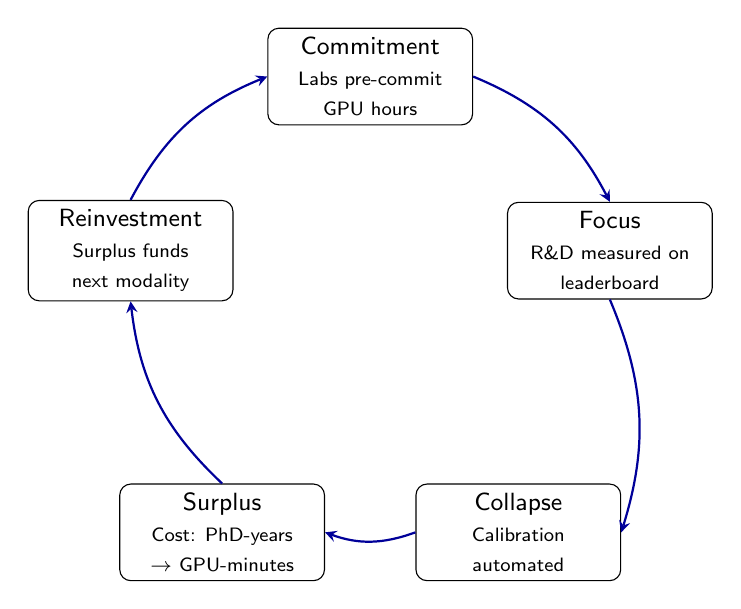
\begin{tikzpicture}[
    node distance=2.4cm,
    every node/.style={
        draw, rounded corners=4pt, align=center,
        minimum width=2.6cm, minimum height=1.1cm,
        font=\small\sffamily
    },
    arrow/.style={->, >=stealth, thick, blue!60!black}
]
  % Nodes arranged in a circle
  \node (commit)    at ( 90:3.2cm) {Commitment\\{\scriptsize Labs pre-commit}\\ {\scriptsize GPU hours}};
  \node (focus)     at ( 18:3.2cm) {Focus\\{\scriptsize R\&D measured on}\\{\scriptsize leaderboard}};
  \node (collapse)  at (-54:3.2cm) {Collapse\\{\scriptsize Calibration}\\{\scriptsize automated}};
  \node (surplus)   at (-126:3.2cm) {Surplus\\{\scriptsize Cost: PhD-years}\\{\scriptsize $\to$ GPU-minutes}};
  \node (reinvest)  at (162:3.2cm) {Reinvestment\\{\scriptsize Surplus funds}\\{\scriptsize next modality}};

  % Circular arrows
  \draw[arrow] (commit.east)    to[bend left=20] (focus.north);
  \draw[arrow] (focus.south)    to[bend left=20] (collapse.east);
  \draw[arrow] (collapse.west)  to[bend left=20] (surplus.east);
  \draw[arrow] (surplus.north)  to[bend left=20] (reinvest.south);
  \draw[arrow] (reinvest.north) to[bend left=20] (commit.west);
\end{tikzpicture}
\caption{%
  \textbf{The Abundance Flywheel.}  Laboratory commitment seeds focused
  R\&D on a shared leaderboard; focused effort collapses calibration
  complexity; collapsed complexity creates cost surplus; surplus funds
  the next modality, reinforcing commitment.}
\label{fig:flywheel}
\end{figure}

\noindent
Each revolution of the flywheel lowers the marginal cost of adding a
modality.  The first 26 modalities required PhD-level effort per
operator; the next 40 should require only GPU-minutes per operator as
automated calibration pipelines mature.

\subsection{The AlphaFold Parallel}

\cref{tab:alphafold} draws an explicit structural comparison between the
AlphaFold ecosystem and PWM.

\begin{table}[t]
\centering
\caption{%
  \textbf{Structural comparison: AlphaFold ecosystem vs.\ PWM.}
  Both systems share the same architecture---a shared task definition,
  a growing observability corpus, and a recurring targeting mechanism---but
  operate in different physical domains.}
\label{tab:alphafold}
\small
\begin{tabular}{@{}lll@{}}
\toprule
\textbf{Dimension} & \textbf{AlphaFold Ecosystem} & \textbf{PWM} \\
\midrule
Purpose
  & Predict protein structure
  & Calibrate \& reconstruct \\
Task Taxonomy
  & Sequence $\to$ 3D coordinates
  & \texttt{ExperimentSpec} $\to$ validated recon.\ \\
Observability
  & PDB (200K+ structures)
  & 26-modality benchmark \\
Targeting
  & CASP (biennial competition)
  & LIP-Arena / CISP \\
\bottomrule
\end{tabular}
\end{table}

\noindent
The analogy is not superficial.  AlphaFold~\cite{jumper2021alphafold} succeeded not because of a
single architectural innovation, but because CASP~\cite{moult2005casp} provided a legible,
recurring, trusted measurement of progress.  PWM aims to provide the
same function for computational imaging through the Computational Imaging
Standardization Project (CISP).

\subsection{Quantified Targets}

\cref{tab:targets} translates the roadmap into measurable milestones
across four key performance indicators.

\begin{table}[t]
\centering
\caption{%
  \textbf{Quantified roadmap targets.}
  L3 and L5 refer to standardization maturity levels as defined in \cref{tab:maturity}.
}
\label{tab:targets}
\small
\begin{tabular}{@{}lccc@{}}
\toprule
\textbf{Metric} & \textbf{Current} & \textbf{L3 Target} & \textbf{L5 Target} \\
\midrule
Recovery ratio        & 0.30--1.0+ & 80\%+    & 95\%+    \\
Oracle gap            & 5--12\,dB  & $\leq$2\,dB   & $\leq$0.5\,dB  \\
Modalities covered    & 64         & 100+     & 200+     \\
Zero-shot generalization & 0\%     & 50\%+    & 90\%+    \\
\bottomrule
\end{tabular}
\end{table}

\noindent
\textbf{Recovery ratio} $\rho$ measures the fraction of the mismatch-induced
degradation that is recovered by operator correction, as defined in
Eq.~\ref{eq:recovery}; the range varies widely by modality (e.g., CASSI $\approx 0.30$, CACTI $> 1.0$).  \textbf{Oracle gap} is the PSNR difference between Scenario~I
(Ideal) and Scenario~III (Corrected).  \textbf{Zero-shot generalization} measures reconstruction
quality on a modality unseen during solver training, evaluated via the
mask-sensitivity spectrum transfer protocol.

\subsection{Three-Phase Roadmap}

We organize the path to standardization into three six-month phases:

\medskip
\noindent
\textbf{Phase 1: Become the Default Evaluation Infrastructure
(Months~1--6).}

\begin{itemize}
  \item \texttt{pip install pwm-eval} --- a one-line entry point for any
        lab to reproduce our 26-modality benchmark.
  \item Three replication packs (CASSI, SPC, CACTI) with frozen operator
        graphs, calibration metadata, and reference reconstructions.
  \item Five external laboratories independently validate the
        four-scenario evaluation protocol.
  \item The mask-sensitivity spectrum adopted as a standard diagnostic
        in at least two peer-reviewed publications outside our group.
\end{itemize}

\medskip
\noindent
\textbf{Phase 2: Launch the CISP Public Competition (Months~7--12).}

\begin{itemize}
  \item \texttt{cisp.pwm.org} --- a public leaderboard with automated
        scoring, inspired by CASP's transparent ranking.
  \item An independent steward board (minimum five institutions) governs
        test-set curation and metric evolution.
  \item Blinded test sets: measurement data released without ground truth;
        reconstructions submitted as sealed \texttt{RunBundle} archives.
  \item Four or more competition tracks spanning snapshot, video,
        spectral, and depth modalities.
\end{itemize}

\medskip
\noindent
\textbf{Phase 3: Become the Action Network (Months~13--18).}

\begin{itemize}
  \item \textbf{Robotic lab API} --- remote-triggered physical
        measurements that close the sim-to-real loop automatically.
  \item \textbf{Compute escrow} --- participating labs pledge GPU hours
        to a shared pool, drawn upon by competition entrants.
  \item \textbf{Calibration-as-a-service API} --- upload raw sensor data,
        receive a calibrated \texttt{OperatorGraph} with uncertainty
        quantification.
  \item \textbf{Outcome-based contracts} --- service-level agreements
        where payment is contingent on achieving a specified PSNR/SSIM
        threshold on the client's measurement.
\end{itemize}

\medskip
\noindent
The foundry window is finite.  Within 18~months, the evaluation norms of
computational imaging will crystallize.  The infrastructure laid in
Phase~1 determines whether those norms are principled, reproducible, and
physics-aware---or whether the field continues to optimize solvers on
idealized simulations while real systems fail silently.
